\documentclass[11pt]{article}
\usepackage[hmargin=1in,vmargin=1in]{geometry}
\usepackage{xcolor}
\usepackage{amsmath,amssymb,amsfonts,url,sectsty,framed,tcolorbox,framed}
\usepackage{graphicx}
\usepackage{tikz}
\usepackage{amsmath}
\usetikzlibrary{shapes, arrows}
\usetikzlibrary{positioning}
\graphicspath{ {./images/} }
\newcommand{\pf}{{\bf Proof: }}
\newtheorem{theorem}{Theorem}
\newtheorem{lemma}{Lemma}
\newtheorem{proposition}{Proposition}
\newtheorem{definition}{Definition}
\newtheorem{remark}{Remark}
\newcommand{\qed}{\hfill \rule{2mm}{2mm}}

\begin{document}
%%%%%%%%%%%%%%%%%%%%%%%%%%%%%%%%%%%%%%%%%%%%%%%%%%%%%%%%%%%%%%%%%%%%%
\rule{\textwidth}{1pt}
\begin{center}
{\bf [CS304] Introduction to Cryptography and Network Security}
\end{center}
Course Instructor: Dr. Dibyendu Roy \hfill Winter 2023-2024\\
Scribed by: Manas Jitendrakumar Ingle (202151086) \hfill Lecture (Week 2)
\\
\rule{\textwidth}{1pt}
%%%%%%%%%%%%%%%%%%%%%%%%%%%%%%%%%%%%%%%%%%%%%%%%%%%%%%%%%%%
\section{Total Permutations[Complexities]}

Let $\{A, B, C, \ldots, Z\}$ be the alphabet.
The encryption function is defined as:\\
$E_s$(M) = S($m_1$)S($m_2$)....S($m_n$) = C \\ 

total possibilities = 26! \\ 
The total number of permutations is $26!$, which is approximately equal to $2^{80}$ possible permutations.\\
The encryption function for a simple affine cipher is given by:
\[ C =  e_{k}(x) = (a \cdot x + b) \mod m \]


 k = (a,b)  where $0 \leq a,b \leq 25$ \\
\begin{itemize}
    \item Modulus $m$ is the size of the alphabet.
    \item $a$ and $b$ are the key parameters of the cipher.
    \item $a$ must be chosen such that $a$ and $m$ are coprime.
\end{itemize}
The total combinations of $a$ and $b$ are $12 \times 26$.

\section{Hill Cipher}
\begin{itemize}
     Secret key $\rightarrow A = (a_{ij})_{n \times n}$ \quad (invertible matrix)
    \\
    \\ $M = m_1 \cdot m_2 \cdot m_3 \ldots m_n$ \quad $\rightarrow$ Plaintext
    \\
    \\ Ciphertext $\rightarrow C = A \cdot M$ \quad (encryption algorithm)
    
    \[ C_j = \sum_{j=1}^{n} a_{ij} \cdot m_j \]
    
    \\ Decryption: $M = A^{-1} \cdot C$
\end{itemize}

\section{Symmetric Key Cryptography}
%\begin{figure}[htbp]
    %\centering
    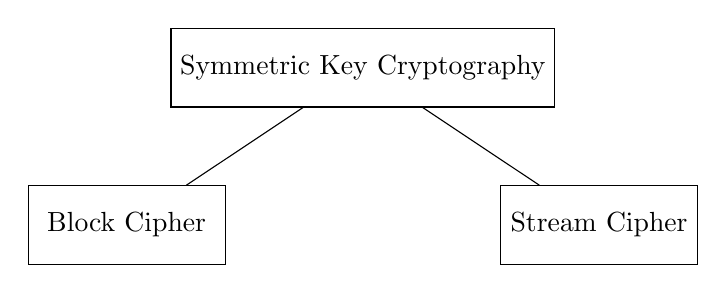
\begin{tikzpicture}[
        level distance=2cm,
        level 1/.style={sibling distance=6cm},
        level 2/.style={sibling distance=3cm},
        level 3/.style={sibling distance=2cm},
        every node/.style={draw, rectangle, minimum width=2.5cm, minimum height=1cm}
    ]
    \node {Symmetric Key Cryptography}
        child { node {Block Cipher} }
        child { node {Stream Cipher} };
    \end{tikzpicture}
    %\caption{Symmetric Key Cryptography: Block Cipher and Stream Cipher}
%\end{figure}

\\

\section{Block Cipher :}
A block cipher is a cryptographic algorithm that processes a fixed-size block of plaintext as a whole
and transforms it into an equally-sized block of ciphertext.\\
It is an Implementation of ECB(electronic code book) mode of operation \\

\\ M = $m_0$ \| $m_1$ \| $m_2$ \|....\| $m_n$  

\\ len(M) = m \quad len($m_i$) = l \hookleftarrow block size \\

\item \textbf{Encryption :}

C = $E_n_c$($m_0$,k) \| $E_n_c$($m_1$,k) \|.....\| $E_n_c$($m_n$,k) \\

ciphertext C = $C_0$ \|  $C_1$ \|  $C_2$ \|... $C_n$ \\ 

$E_n_c$(m,k) = C  \quad  $E_n_c$ = M\timesK \\

\item \textbf{Decryption :}

M = Dec($C_0$,k) \| Dec($C_1$,k) \|......\| Dec($C_n$,k) \\ 

M = $m_0$ \| $m_1$ \| $m_2$ \quad where len($m_0$) = len($m_1$) = n and len($m_2$) = l \\

length = 2n+l \quad where l \leq n \\

$C_0$ = $E_n_c$($m_0$,k),\quad $C_1$ = $E_n_c$($m_1$,k),\quad 
$C_2$ = $E_n_c$($m_2$ \| $0^n^-^l$,k) \\

C = $C_0$ \|  $C_1$ \|  $C_2$  \quad where $C_2$ \rightarrow $m_2$ \| 0....0 \hookleftarrow padding\quad to\quad make\quad length\quad equal \\


\section{Product Cipher :}
It combines two or more transformations in a manner intending that the resulting ciphers is more secure than it's individual components.\\

\item \textbf{Example: Substitution Permutation Network (SPN) } \\

Plaintext P : \{0,1\}^{m \cdot r} \rightarrow \{0,1\}^{m \cdot r} \\

Ciphertext S : \{0,1\}^n \rightarrow \{0,1\}^m  \\


\begin{tikzpicture}
\draw[->] (0,0) -- (1,0);
\node at (-0.25,0) {p};
\node[draw, rectangle, minimum width=8cm, minimum height=0.5cm, align=center] at (5.5,0) 
{m\textsubscript{r}};
\node at (2.3,2.5) {n};
\draw[->] (2,3) -- (2,2);
\node[draw, rectangle, minimum width=0.5cm, minimum height=0.5cm, align=center] at (2,1.5) 
{s};
\node at (2.3,0.8) {m};
\draw[->] (2,1) -- (2,0);

\node at (4.3,2.5) {n};
\draw[->] (4,3) -- (4,2);
\node[draw, rectangle, minimum width=0.5cm, minimum height=0.5cm, align=center] at (4,1.5) 
{s};
\node at (4.3,0.8) {m};
\draw[->] (4,1) -- (4,0);

\node[] at (6, 1.5){.... r ....};

\node at (8.3,2.5) {n};
\draw[->] (8,3) -- (8,2);
\node[draw, rectangle, minimum width=0.5cm, minimum height=0.5cm, align=center] at (8,1.5) 
{s};
\node at (8.3,0.8) {m};
\draw[->] (8,1) -- (8,0);
\end{tikzpicture}
    
\section{Fiestel Network}
There are several steps in making a fiestel network.
\begin{itemize}
    \item The data is divided into equal left and right part.
    \item In the next iteration the right part from the previous iteration becomes the left part of the next iteration
    \item For the right part
    \begin{itemize}
        \item We have a function F that takes 2 parameters, a piece of data and a secret key k.
        \item We apply the function on right part of the previous iteration and a secret key k
        \item then we take the output and xor it with the left part of the previous part of the iteration. This becomes the right part of the next iteration.
    \end{itemize}
\end{itemize}
Below image explains the above steps
\item \textbf{Encryption :} \\
f :  \{0,1\}^n \times \{0,1\}^k \rightarrow  \{0,1\}^n

$L_1$ = $R_0$ \\
$R_1$ = $L_0$ \oplus f($R_0$, k) \\

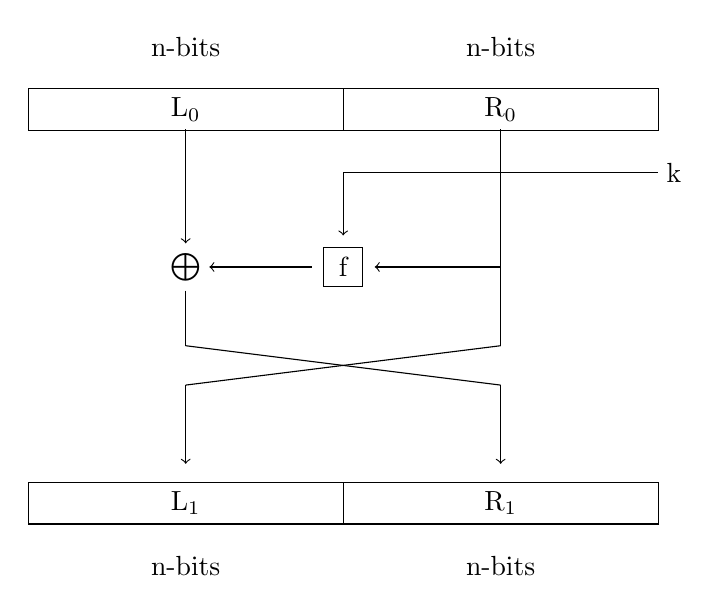
\begin{tikzpicture}
\node at (0,0.8) {n-bits};
\node at (4,0.8) {n-bits};
\node[draw, rectangle, minimum width=4cm, minimum height=0.5cm, align=center] at (0,0) 
{L\textsubscript{0}};
\node[draw, rectangle, minimum width=4cm, minimum height=0.5cm, align=center] at (4,0) 
{R\textsubscript{0}};
\draw[->] (0,-0.25) -- (0,-1.7);
\node at (0,-2) {$\bigoplus$};
\draw[-] (4,-0.25) -- (4,-2);

\node[draw, rectangle, minimum width=0.5cm, minimum height=0.5cm, align=center] at (2,-2) 
{f};
\draw[->] (4,-2) -- (2.4,-2);
\draw[->] (1.6,-2) -- (0.3,-2);
\draw[->] (2,-0.8) -- (2,-1.6);
\draw[-] (2,-0.8) -- (6,-0.8);
\node at (6.2,-0.8) {k};
\draw[-] (0,-2.3) -- (0,-3);

\node[draw, rectangle, minimum width=4cm, minimum height=0.5cm, align=center] at (0,-5) 
{L\textsubscript{1}};
\node[draw, rectangle, minimum width=4cm, minimum height=0.5cm, align=center] at (4,-5) 
{R\textsubscript{1}};
\node at (0,-5.8) {n-bits};
\node at (4,-5.8) {n-bits};

\draw[-] (0,-3) -- (4, -3.5);
\draw[->] (4,-3.5) -- (4, - 4.5);
\draw[-] (4,-2) -- (4, -3);
\draw[-] (4,-3) -- (0, - 3.5);
\draw[->] (0,-3.5) -- (0, - 4.5);

\end{tikzpicture}\\
This Image shows Demonstration of a single Round..Such Multiple(r) rounds can  exist. 
\item \textbf{Decryption :}
$L_0$ = $R_1$ \oplus f($L_1$,k)

\section{Iterated Block Cipher}
It is a Block Cipher where involving the sequential repetition of an internal function called as round function where tha parameters include the number of rounds 'r', the block size 'n' and bit size '$x^k$' of the input key 'k' from which 'r' subkeys '$k_i$' (round keys) are derived.

\item \textbf{Example: 2-round iterated block cipher encryption} \\

\item \textbf{Encryption:}
F($k_1$,P) \rightarrow $C_1$ \rightarrow F($k_2$,$C_1) = C \\
Where P \rightarrow Plaintext \quad C \rightarrow Ciphertext \\

rounds = 2 \\ 
round keys = $k_1$, $k_2$ \\

k \rightarrow G(k) \rightarrow $k_1$, $k_2$ \quad Where G is Key Scheduling Algorithm \\

\item\textbf{Decryption:}
C \rightarrow $F^-^1$($C_1$,$k_2$) \rightarrow $C_1$ \rightarrow $F^-^1$($C_1$,$k_1$) = plaintext P \\ 



\section{Data Encryption Standard (DES):}
\begin{itemize}
\item Designed by IBM it is based on Fiestel network. DES is an iterated block cipher with 16 rounds. 
\item It has a secret key of 64-bit and the plaintext block size of 64-bit as well.
\item In the 64-bit key, there are 8 parity check bits. So, those 8 bits are decided by the remaining 56 bits. Which means that the ctual key is ascutally only 56-bit
\item \textbf{Encryption :} \\
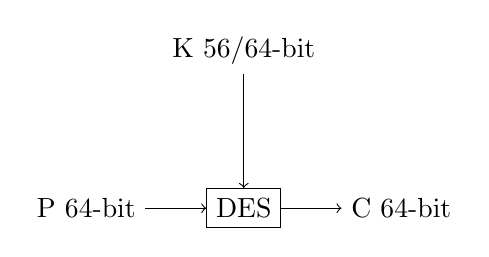
\begin{tikzpicture}[node distance=2cm]
\node (P) {P 64-bit};
\node[draw, rectangle, minimum width=0.5cm, minimum height=0.5cm, align=center] (DES) [right of=P] {DES};
\node (C) [right of=DES] {C 64-bit};
\node (K) [above of=DES] {K 56/64-bit};
\draw[->] (P) -- (DES);
\draw[->] (DES) -- (C);
\draw[->] (K) -- (DES);
\end{tikzpicture}





\item \textbf{Decryption :} \\
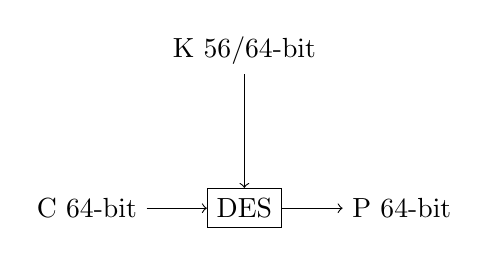
\begin{tikzpicture}[node distance=2cm]
\node (C) {C 64-bit};
\node[draw, rectangle, minimum width=0.5cm, minimum height=0.5cm, align=center] (DES) [right of=C] {DES};
\node (P) [right of=DES] {P 64-bit};
\node (K) [above of=DES] {K 56/64-bit};
\draw[->] (C) -- (DES);
\draw[->] (DES) -- (P);
\draw[->] (K) -- (DES);
\end{tikzpicture}

\item \textbf{Key scheduling algorithm for 64-bit key : } \\

Keys K \rightarrow $k_1$, $k_2$, $k_3$...., $k_1_6$ \\

Where every $K_i$ is of 48-bit \\

input P (64-bit) \quad IP(initial permutation) : \{0,1\}^{64} \rightarrow \{0,1\}^{64} \\



\end{itemize}


\end{document}